\documentclass[11pt]{article}
\usepackage{amssymb}

\usepackage[T1]{fontenc}
\usepackage{inconsolata}
\usepackage{textcomp}
\usepackage{listings}
\usepackage{color}
\usepackage[normalem]{ulem}
\usepackage{float}
\usepackage{graphicx}
\usepackage{amsmath}
\usepackage{mathtools}
\graphicspath{ {figs/} }
\usepackage[hidelinks]{hyperref}
\usepackage{xcolor,soul,lipsum}
\newcommand{\myul}[2][black]{\setulcolor{#1}\ul{#2}\setulcolor{black}}
\usepackage{enumitem}
\usepackage[bottom]{footmisc}

\usepackage[utf8]{inputenc} % this is needed for umlauts
\usepackage[ngerman]{babel} % this is needed for umlauts
\usepackage[T1]{fontenc}    % this is needed for correct output of umlauts in pdf
\usepackage{amssymb,amsmath,amsfonts} % nice math rendering
\usepackage{braket} % needed for \Set
\usepackage{caption}
\usepackage{algorithm}
\usepackage[noend]{algpseudocode}

\DeclareCaptionFormat{myformat}{#3}
%\captionsetup[algorithm]{format=myformat}


\makeatletter
\DeclareUrlCommand\ULurl@@{%
  \def\UrlFont{\ttfamily\color{blue}}%
  \def\UrlLeft{\uline\bgroup}%
  \def\UrlRight{\egroup}}
\def\ULurl@#1{\hyper@linkurl{\ULurl@@{#1}}{#1}}
\DeclareRobustCommand*\ULurl{\hyper@normalise\ULurl@}
\makeatother


\makeatletter
\renewcommand\thesection{}
\renewcommand\thesubsection{}
\makeatother

\textwidth=6in
\oddsidemargin=0.25in
\evensidemargin=0.25in
\topmargin=-0.1in
\footskip=0.8in
\parindent=0.0cm
\parskip=0.3cm
\textheight=8.00in
\setcounter{tocdepth} {3}
\setcounter{secnumdepth} {2}
\sloppy

\begin{document}

\setlength{\oddsidemargin}{.25in}
\setlength{\evensidemargin}{.25in}
\setlength{\textwidth}{6in}
\setlength{\topmargin}{-0.4in}
\setlength{\textheight}{8.5in}

\newcommand{\handout}[5]{
   \renewcommand{\thepage}{#1-\arabic{page}}
   \noindent
   \begin{center}
   \framebox{
      \vbox{
    \hbox to 5.78in { {\bf Reinforcement Learning} \hfill #2 }
       \vspace{4mm}
       \hbox to 5.78in { {\Large \hfill #5  \hfill} }
       \vspace{2mm}
       \hbox to 5.78in { {\it #3 \hfill #4} }
      }
   }
   \end{center}
   \vspace*{4mm}
}
\newcommand{\exercise}[4]{\handout{#1}{#2}{Lecturer:#3}{TA: #4}{Exercise #1}}
\newenvironment{remark}{\noindent{\bf Remark}\hspace*{1em}}{\bigskip}

%%%%%%%%%%%%%%%%%%%%%%%%%%%%%%%%%%%%%%%%%%%%%%%%%%%%%%%%%%%%%%%%%%%%%%%%%%%%%%%%%%%%%

\exercise{2}{March 13, 2022}{Yishay Mansour}{Asaf Cassel}

\lstdefinestyle{myLuastyle}
{
  language         = {[5.2]Lua},
  showstringspaces = false,
  upquote          = true,
  basicstyle=\ttfamily,
  keywordstyle=\color{blue}\ttfamily,
  stringstyle=\color{red}\ttfamily,
  commentstyle=\color{green}\ttfamily,
  morecomment=[l][\color{magenta}]{\#}
}

\lstset{style=myLuastyle}


Due date: March 28, 2022

\section{Theory}

% \subsection{Question 1}

% Consider a multiplicative model, where the return function of the reward sequence $r_1, . . . , r_N$ is  $\prod_{i=1}^{N}r_i$, $r_i>0$. Develop an algorithm that evaluates a given deterministic Markovian policy for such a return function.
\subsection{Question 1}
Consider a Markov chain with states $S=\{1,2,3,4\}$ and the following transition matrix:
\[
P= \begin{pmatrix}
0 & 1 & 0 & 0\\
0 & 0 & 1/3 & 2/3\\
1 & 0 & 0 & 0\\
0 & 1/2 & 1/2 & 0\\
\end{pmatrix}\]

\begin{enumerate}
\item Draw the state transition diagram.
\item State the communicating classes. Is the chain irreducible?
\item Calculate $d_i$, the period of each state. Is the chain aperiodic?
\item If possible, find the invariant distribution.
\item For every state $i\in S$, calculate $E[T_i]$, the expected return time to state $i$ (hint: use the previous clause). Which states are recurrent? Classify each recurrent state as null or positive.
\item Write a new transition matrix $P'$ so that $E[T_1]=3$ and $d_1=3$. Calculate $p^{m}_{1,1}$ as a function of $m$ for that transition matrix, given that $1$ is the initial state.
\end{enumerate}
\newpage

\subsection{Question 2}
An MDP is represented by a bidirectional cycle of size $2k$, where each node $\in\{0,\dots,2k-1\}$ is a state. The MDP starts at state $k$.
There are two available actions: CW (clockwise) and CCW (counter-clockwise), both are deterministic. (CW turns state $i$ into state $i+1 mod\; 2k$ and CCW turns every state $i$ to $i-1 mod\; 2k$.)\\
The reward from each action state $(s,a)$ is $0$ for all states but state $0$ that receives a (running) reward of $1$ (for CW and CCW).\\
The return is discounted with parameter $\gamma<1$.

\begin{figure}[h]
\centering
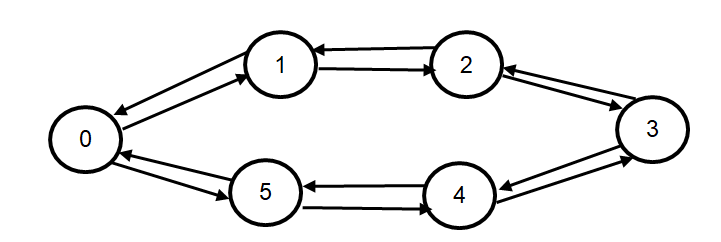
\includegraphics[width=6cm,height=6cm,keepaspectratio]{mdp cw ccw fixed}
\end{figure}

\begin{enumerate}
\item Write a formal MDP for this problem (i.e., $\mathcal{S}, {\mathcal{A}}, \mathcal{P}, {\mathcal{R}}$ and $s_0 $).
\item What is the optimal policy $\pi^*$?
\item After one iteration of the Value Iteration algorithm (where all states start with a value of $0$), which states change their value after one iteration? what are the new values?
\item Which states change their value after two iterations? what are the new values?
\item For $k=2$ ($4$ states), calculate $V^*(s)$ for every $s\in \mathcal{S}$ (as a function of $\gamma$).

\end{enumerate}

\newpage
\subsection{Question 3}
Consider the following digit game. We have $N+1$ slots, marked by $0$ to $N$. At each round (of $N+1$ rounds) a random digit is chosen. (I.e., a random digit from $\{0,1,...,9\}$.) We can put the digit in one of the unoccupied slots, and that slot becomes occupied. %(Namely, after $k$ digits our actions are $\{1, \ldots , N+1-k$, which is indices of the unoccupied slot.) 
Our aim is to maximize the expected value of the sequence of digits, when viewed as a number. (I.e. if we have $d_i$ in slot $i$ then the final value is  $\sum_{i=0}^{N}d_i10^i$.)

Example: Suppose $N=2$. At the beginning we have three empty slots. Let us denote an empty slot by ×, then we have × × ×. Suppose the first digit is 5, and we decide to put it in the second slot, then we have ×5×. Suppose the second digit is 4 and we decide to put it in the first slot, we have ×54. Finally, the last digit is 4 again, and our final number is 454.

\begin{enumerate}
\item Build an MDP for this problem. (Hint: you may incorporate the random digit in the state.)
\item Show that the decision of the optimal policy depends only on the number of empty slots and the current random digit $d_i$. For example, in round $2$, the game is in $d_0$ × ×/ × $d_0$ × /  × × $d_0$ and a current digit is $d_1$, the optimal policy will put $d_1$ in  $d_0$ $d_1$ ×/ $d_1$ $d_0$ × /  $d_1$ × $d_0$ respectively or $d_0$ × $d_1$/ × $d_0$ $d_1$ /  × $d_1$ $d_0$ for every $d_0,d_1\in \{0,1,...,9\}$.
\item Compute the optimal policy for $N=2$. (I.e the number has three digits.)
\end{enumerate}

\subsection{Question 4}
Let $M$ be an MDP, defined by $(S,A,P,S_0,r)$.\\
Let $T$ be the following operator for $V\in\mathbb{R}^{|S|}$:
\[
\left( {{TV}} \right)\left( s \right) =\frac{1}{|A|}\sum_{a\in A} \left( {r\left( {s,a} \right) + \gamma {\sum _{s' \in S}}p\left( {s'|s,a} \right)V\left( {s'} \right)} \right)
\]
Show that $T$ is a $\gamma$-contracting with respect to the max-norm.

% \newpage
% \section{Programing}

% \subsection{Intro}
% The following questions will use the Frozen Lake environment, a simple gridworld MDP that is taken from gym and slightly modified for this assignment. In this MDP, the agent must navigate from the start state to the goal state on a 4x4 grid, with stochastic transitions. You can read more about the environment here: \url{https://gym.openai.com/envs/FrozenLake-v0/}.

% You are provided with template python script in which you should implement the algorithm: \text{\ttfamily value\_iter.py} and \text{\ttfamily policy\_iter.py}.

% An example episode is given below, the agent falls into a hole after two timesteps. Note the stochasticity--on the first step, the DOWN action is selected, but the agent moves to the right.

% \begin{figure}[h]
% \centering
% 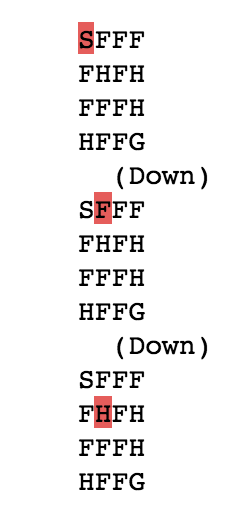
\includegraphics[width=6cm,height=6cm,keepaspectratio]{figs/frozenlake}
% \end{figure}

% \newpage

% \subsection{Question 1: Value Iteration}
% In this problem, you will implement value iteration, which has the following pseudocode:

% \begin{algorithm}[h]
% \begin{algorithmic}
% \State Initialize $V^{(0)}(s)=0$, for all $s$
% \For{$i=0, 1, 2, \dots$}
% 	\For {for all $s \in S$}
% 	\State $V^{(i+1)}(s) = \max_a \sum_{s'} P(s,a,s') [ R(s,a,s') + \gamma V^{(i)}(s')]$
%     \EndFor
% \EndFor
% \end{algorithmic}        
% \caption{Value Iteration}
% \label{alg:value-iteration}
% \end{algorithm}

% We additionally define the sequence of greedy policies $\pi^{(0)}, \pi^{(1)}, \dots, \pi^{(n-1)}$, where
% \begin{equation}
% \pi^{(i)}(s) = \arg \max_a \sum_{s'} P(s,a,s') [ R(s,a,s') + \gamma V^{(i)}(s')]
% \end{equation}

% Your code will return two lists: $[V^{(0)}, V^{(1)}, \dots, V^{(n)}]$ and $[\pi^{(0)}, \pi^{(1)}, \dots, \pi^{(n-1)}]$

% \textul{\textbf{Note 1}}: Choose the lower-index action to break ties in $\arg \max_a$. This is done automatically by np.argmax. This will only affect the "\# chg actions" printout below--it won't affect the values computed.

% \textul{\textbf{Note 2}}: Make a copy of your value function each iteration and use that copy for the update--don't update your value function in place. 
% Updating in-place is also a valid algorithm, sometimes called Gauss-Seidel value iteration or asynchronous value iteration, but it will cause you to get different results than our reference solution.

% \begin{enumerate}
% \item Implement the relevant code in the attached \text{\ttfamily{value\_iter.py}} code. The relevant locations are marked with \text{\ttfamily{REPLACE THIS LINE WITH YOUR CODE}} comment. 
% \item Submit: (i) plot of the optimal policy at each iteration and (ii) plot of each state value as a function of iterations (different curve for each value, same figure). The script already contains the code for (i).
% \end{enumerate}

% Submit your modified code, iteration table outputted by the code and plots. 

% \newpage

% \subsection{Question 2: Policy Iteration}

% The next task is to implement exact policy iteration (PI), which has the following pseudocode::

% \begin{algorithm}[h]
% \begin{algorithmic}
% \State Initialize $\pi_0$
% \For{$i=0, 1, 2, \dots$}
%   \State Compute the state-value function $V^{\pi_{n}}$
%   \State Using $V^{\pi_{n}}$, compute the state-action-value function $Q^{\pi_{n}}$
%   \State Compute new policy $\pi_{n+1}(s) = \operatorname*{argmax}_a Q^{\pi_{n}}(s,a)$
% \EndFor
% \end{algorithmic}        
% \caption{Policy Iteration}
% \label{alg:value-iteration}
% \end{algorithm}

% You will implement the first and second steps of the loop using the attached \text{\ttfamily policy\_iter.py}.

% Your code will return two lists: $[V^{(0)}, V^{(1)}, \dots, V^{(n)}]$ and $[\pi^{(0)}, \pi^{(1)}, \dots, \pi^{(n-1)}]$

% \begin{enumerate}
% \item Implement the function called \text{\ttfamily compute\_vpi} that computes the state-value function $V^\pi$ for an arbitrary policy $\pi$ . Recall that $V^\pi$ satisfies the following linear equation:

% \begin{equation}
% V^{\pi}(s) = \sum_{s'} P(s,\pi(s),s')[ R(s,\pi(s),s') + \gamma V^{\pi}(s')]
% \end{equation}

% You can solve a linear system in your code. (Find an exact solution, e.g., with \text{\ttfamily np.linalg.solve}). As before, look for the \text{\ttfamily REPLACE THIS LINE WITH YOUR CODE} comment.

% \item Implement the function called \text{\ttfamily compute\_qpi} computes the state-action value function $Q^{\pi}$, defined as follows
% \begin{equation}
% Q^{\pi}(s, a) = \sum_{s'} P(s,a,s')[ R(s,a,s') + \gamma V^{\pi}(s')]
% \end{equation}
% As before, look for the \text{\ttfamily REPLACE THIS LINE WITH YOUR CODE} comment.

% \item Using the functions you implemented in parts (1) and (2) implement the function called \text{\ttfamily policy\_iteration} which implements policy iteration. This time, look for the \text{\ttfamily YOUR CODE HERE} comment.


% \end{enumerate}

% Submit your modified code, iteration table outputted by the code and value plot. 


\end{document}